\documentclass[11pt, a4paper, table]{article}
\usepackage[dvipsnames]{xcolor}
\usepackage{tikz}
\usepackage{amsmath}
\usepackage[dutch]{babel}
\usepackage[latin1]{inputenc} 
\usepackage{float}
\usepackage{algpseudocode}
\usepackage{algorithm}
\usepackage{textcomp}
\usepackage{amsthm}
\usepackage{rotating}
\usepackage[section]{placeins}




\usepackage[skins]{tcolorbox}
\makeatletter
\newenvironment{algoritme}[1][H]{%
	\renewcommand{\ALG@name}{Algoritme}% Update algorithm name
	\renewcommand{\algorithmicrequire}{\textbf{Input:}}
	\renewcommand{\algorithmicensure}{\textbf{Output:}}
	\begin{algorithm}[#1]%
	}{\end{algorithm}}
\makeatother

\theoremstyle{definition}
\newtheorem{opgave}{Opgave}

\begin{document}
	\title{Project Gretige Algoritmen}
	\author{Jarre Knockaert}
	\maketitle
	
\thispagestyle{empty}
\newpage
\pagenumbering{arabic}

\section{Theoretische vragen}
\begin{opgave}
	Indien er 2 naburige toppen v en w een grote bedekking leveren, zal de top v met de hoogste graad worden toegevoegd aan de dominante verzameling en de buren zullen worden verwijderd. Het zou echter beter zijn om zowel v en w toe te voegen aan de dominante verzameling, want w leidt ook tot een hoge toename van de bedekking van de dominante verzameling. 
	Een voorbeeld van dergelijk geval, een graaf waarbij het algoritme zeer slecht presteert, zie je op figuur \ref{fig:worstcase}. Als we het algoritme uitvoeren op de graaf gebeurt het volgende:
	\begin{itemize}
		\item Neem top v = $4k+1$ met hoogste graad: $2k-1$. (Dit kon evengoed top $4k+2$ zijn, aangezien zijn graad gelijk is.)
		\item Voeg v toe aan de dominante lijst D. 
		\item Verwijder v en al zijn buren (top $1$ tot en met top $2k$) uit de graaf G. Nu bevat de G nog $2k-1$ toppen (top $2k+1$ tot en met top $4k$).
		\item De resterende toppen uit de graaf hebben elk graad 0 en zijn ge\"{i}soleerde toppen. (Aangezien hun enige buur werd verwijderd uit de graaf.) Voor elke top w van $2k+1$ tot en met top $4k$ gebeurt nu het volgende:
		\begin{itemize}
			\item Neem de top w. Aangezien elke top graad 0 heeft maakt het niet uit welke top we uit de graaf kiezen. Hun graad is (en blijft) gelijk aan elkaar. 
			\item Voeg w toe aan D. 
			\item Verwijder w uit G. De top w is ge\"{i}soleerd en dus er zullen ook geen extra toppen uit de graaf verwijderd worden. 
		\end{itemize}
	\end{itemize}
	In totaal werden $2k$ toppen toegevoegd aan de dominante lijst: top $4k+1$ en top $2k+1$ tot en met top $4k$. De minimale dominante verzameling bevat echter enkel de 2 toppen $4k+1$ en $4k+2$. 
	Het resultaat van het algoritme is een dominante verzameling met $\frac{2k}{2}=k$ keer meer toppen meer dan de optimale dominante verzameling. 
	\begin{figure}[H]
	%\centering
		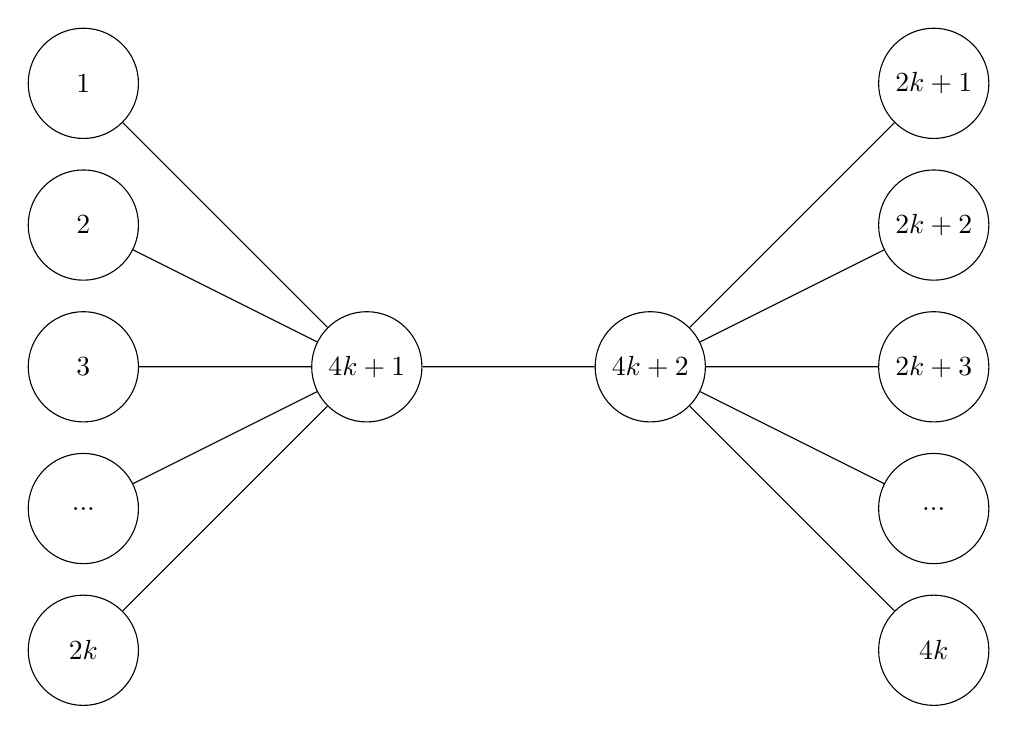
\begin{tikzpicture} 
		[main node/.style={circle, draw, minimum width=1.4cm, minimum height=1.4cm}, scale=1.8]
		\def\length{3}
			\foreach \a in {1,2,...,\length}{
				\node[main node]  (\a) at (0, 2+\length-\a) {$\a$};
				\node[main node]  (2k+\a) at (6, 2+\length-\a) {$2k+\a$};
			}
			\node[main node]  (leftdots) at (0, 1) {...};
			\node[main node]  (rightdots) at (6, 1) {...};
			\node[main node]  (2k) at (0, 0) {$2k$};
			\node[main node]  (4k) at (6, 0) {$4k$};
			\node[main node] (4k+1) at (2,2) {$4k+1$}; 
			\node[main node] (4k+2) at (4,2) {$4k+2$}; 
	
			\path (leftdots) edge node {} (4k+1);
			\path (rightdots) edge node {} (4k+2);
			\path (4k+1) edge node {} (4k+2);
			\path (2k) edge node {} (4k+1);
			\path (4k) edge node {} (4k+2);
			\foreach \a in {1,2,...,\length}{
				\path (\a) edge node {} (4k+1);
				\path (2k+\a) edge node {} (4k+2);
			}
		\end{tikzpicture}
		\caption{Een graaf waarbij het algoritme slecht presteert.}
		\label{fig:worstcase}
	\end{figure}
\end{opgave}
\begin{opgave}
\end{opgave}
\begin{opgave}
		Hier volgt een uitvoerige bespreking van de algoritmes. 
		\begin{tcolorbox}[blanker,float=tbp, grow to left by=2cm,grow to right by=2cm]
		\begin{algoritme}
			\caption{Dominante verzameling van vlakke grafen (met optimalisaties)}
			\begin{algorithmic}[1]
				\Require Een planaire graaf G(V(G),E(G))
				\Ensure Een dominante verzameling D
				\State $totalCoverage \gets 0$
				\State Count-sort V(G) op basis van de graad van de toppen\label{sortoperation}
				\ForAll{$v\ |\ v \in V(G) \land deg(v)=1$}\Comment{Optimalisatie 1}\label{startoptimalizationloop1}
					\State Neem $w\ |\ wv \in E(G)$\Comment{v heeft \'{e}\'{e}n buur}
					\If{w nog niet bezocht $\land\ coverage(w) > 0$}
						\State $D \gets D \cup \{w\}$
						\State bezoek w 
						\State $totalCoverage \gets totalCoverage+1$
						\State $coverage(w) \gets 0$
					\EndIf 
					\ForAll {$u\ |\ u \in V(G) \land uw \in E(G)$}
						\State $coverage(u) \gets coverage(u) - 1$
						\If{u niet bezocht}
							\State bezoek u
							\State $totalCoverage \gets totalCoverage + 1 $
						\EndIf
					\EndFor
					\If{$totalCoverage = |V(G)|$}
						\State Stop de foreach loop
					\EndIf 
				\EndFor\label{endoptimalizationloop1}
				\ForAll{ $minimum \in \{6, 5,...,0\}$} \Comment{Optimalisatie 2}\label{startoptimalizationloop2}
					\State $i \gets 0$
					\While{$totalCoverage < |V(G)| \land i<|V(G)|$}\label{startactualalgorithmloop}
					\State $v \gets v_i \in V(G)$
						\If{$coverage(v) > 0$}
							\State Neem $max\ |\ (\forall u \in \{v\} \cup N_G(v)) \land (max \ne u) \Rightarrow coverage(max)>coverage(u))$
							\If{$coverage(max) > minimum$}
								\State actualCoverage $\gets \{w\ |\ w \in N_G(max) \land w\ niet \  bezocht\}|$\label{neighbourloop2}
								\If{$actualCoverage > minimum$}
									\State $totalCoverage \gets totalCoverage + actualCoverage$
									\State $coverage(max)  \gets 0$
									\State $ D \cup \{max\}$
									\State Bezoek max en zijn buren\label{neighbourloop3}
								\EndIf 
							\EndIf
						\EndIf
						\State $i \gets i+1$
					\EndWhile\label{endactualalgorithmloop}
				\EndFor\label{endoptimalizationloop2}
				
			\end{algorithmic}
		\end{algoritme}
		\end{tcolorbox}

		Enkele belangrijke vermeldingen bij algoritme 1. 
		\begin{itemize}
		\item Een buur is bezocht indien de top element is van de dominante verzameling of indien een buur van deze top element is van de dominante verzameling.
		\item De bedekking/coverage van een top is de bovengrens van het aantal onbezochte buren.
		\item De werkelijke bedekking/coverage van een top is gelijk aan het aantal onbezochte buren. 
		\item De coverage van een verzameling van toppen is een som van de coverage van alle buren.
		\item De totalCoverage is de de som van de coverage van alle buren. Indien de coverage gelijk is aan |V(G)|, dan is de dominante verzameling klaar. 
		\item De variabele, minimum, stelt een ondergrens voor van de werkelijke bedekking die een top moet bieden aan de graaf voor de top kan toegevoegd worden aan de dominante verzameling.
		\end{itemize}
		
		Algoritme 1 loopt in lineaire tijd. Ik zal de verschillende delen van het algoritme bespreken om de complexiteit te verklaren. Beschouw bij deze analyse n als het aantal toppen. De lijnen die niet besproken worden zijn triviaal en hebben constante tijd $\Theta(1)$.
		\begin{itemize}
			 \item Lijn \ref{sortoperation}: Hier wordt counting sort toegepast op de toppenverzameling om deze te ordenen op basis van hun graad. De complexiteit van counting sort is O(n+k). Hier is k (de graad) begrensd door n-1. De totale complexiteit is hier $O(2n-1)$.
			 \item Lijn \ref{startoptimalizationloop1} $\rightarrow$ \ref{endoptimalizationloop1}: Er wordt ge\"{i}tereerd over de toppen met graad 1. Dit zijn er hoogstens n-1. Stel v de top met graad 1 en w de enige buur van deze top. 
			 Er wordt ge\"{i}tereerd over alle aanliggende bogen van w. Elke boog wordt hoogstens 2 keer bekeken. De reden hiervan is dat de top w maar \'{e}\'{e}n keer wordt genomen als naburige top van top v met graad 1. Er wordt eenmalig ge\"{i}tereerd over al zijn aanliggende bogen. De aanliggende bogen kunnen echter nog maar \'{e}\'{e}n keer bekeken worden bij het itereren over de bogen van een buur van een andere top met graad 1. 
			 Elke boog kan dus hoogstens 2 keer bekeken worden bij het itereren over de bogen van toppen die een buur zijn van een top met graad 1. De boog van een top met graad 1 wordt ook maar twee keer bekeken, eens om zijn buur te bepalen, nogmaals tijdens het itereren over de bogen van zijn buur. In het geheel wordt dus elke boog hoogstens 2 keer bekeken. 
			 In een planaire graaf zijn er hoogstens $3n-6$ bogen. De volledige lus is dus lineair in het aantal toppen. De totale complexiteit is hier $O(2*(3n-6)) = O(6n-12)$
			\item Lijn \ref{startoptimalizationloop2}: De for lus wordt precies 7 keer uitgevoerd. De totale complexiteit is hier 
			$O(7*(complexiteit\ van\ elke\ iteratie))$
			\item Lijn \ref{startactualalgorithmloop} $\rightarrow$ \ref{endactualalgorithmloop} : De complexiteitsanalyse van deze lus is gelijkaardig aan de complexiteitsanalyse van lijn \ref{startoptimalizationloop1} $\rightarrow$ \ref{endoptimalizationloop1}. De buitenste lus gebeurt hoogstens n keer. (i stelt de index voor van de huidige top.) Eerst wordt lokaal gezocht naar het maximum via de aanliggende bogen van top v. Elke aanliggende boog wordt nu hoogstens \'{e}\'{e}n keer bekeken op lijn \ref{neighbourloop1}. Dit wordt hoogstens 1 keer uitgevoerd bij elke top, een boog heeft 2 eindpunten, dus wordt hoogstens 2 keer vanuit elk eindpunt bekeken. Vervolgens op lijn \ref{neighbourloop2} wordt opnieuw ge\"{i}tereerd over de bogen van de node max. Een node kan hoogstens \'{e}\'{e}n keer als max genomen worden. $n-2$ nodes kunnen als maximum gekozen worden. Elke boog kan op deze lijn opnieuw hoogstens 2 keer overlopen worden, 1 keer vanuit zijn beide eindpunten, indien beide eindpunten eens de max node zijn. Als laatste wordt ook op lijn \ref{neighbourloop3} nogmaals over dezelfde bogen als op lijn \ref{neighbourloop2} ge\"{i}tereerd. Elke boog wordt op deze lijn dus ook hoogstens 2 keer bekeken. In totaal wordt deze boog dus hoogstens 4 keer bekeken. Nu kan dus elke boog hoogstens 6 keer bekeken worden in de volledige while-lus. In een planaire graaf zijn er hoogstens $3n-6$ bogen. De volledige lus is dus lineair in het aantal toppen. De totale complexiteit is hier $(O(6*(3n-6)))=O(18n-36)$.
		
		
		De volledige complexiteit is nu: 
		\[(2n-1)+(6n-12)+(7*(18n-36))=134n-256\ (=O(n))\]
		
			Het algoritme is gretig aangezien we itereren over de toppen en telkens lokaal zoeken naar de best toe te voegen top. De top die het beste lijkt wordt vervolgens toegevoegd aan de lijst en zo wordt (het grootste deel van de) verzameling opgebouwd. Het algoritme is nu dus per definitie gretig aangezien het bij elk stadium naar het lokale optimum zoekt.
			Het gretig algoritme heeft 5 onderdelen: (De 5 onderdelen van een gretig algoritme volgens wikipedia.)
			\begin{itemize}
				\item Een kandidaatverzameling: de verzameling D
				\item Een selectie functie: het lokaal zoeken naar de optimale top
				\item Een haalbaarheidsfunctie het vergelijken van de eigenlijke bedekking van een top met 0. 
				\item Een objectieve functie: het toevoegen van het maximum aan de verzameling D
				\item Een oplossing functie: het vergelijken van de actualCoverage met |V(G)|
			\end{itemize} 
			 Vooraf worden ook toppen toegevoegd die buur zijn van een top met graad 1. Hier wordt niet gekeken naar de bedekking van de top. Het is een optimalisatie en wordt voorafgaand aan het werkelijk gretig algoritme uitgevoerd. 
		\end{itemize}
\end{opgave}
\section{Implementatie}
\subsection{Dominantie in vlakke grafen}
\subsubsection{Algoritme en implementatie}
\paragraph{Opslag van de graaf}
Een graaf is een aparte klas en bevat de volgende 3 datastructen:
\begin{itemize}
	\item Een array met bogen
	\item Een array met toppen
	\item Een SortedNodeArray (eigen klasse)
\end{itemize}
De eerste 2 datastructuren zijn redelijk voor de hand liggend. Aangezien initieel telkens het aantal bogen en toppen geweten is uit een graaf is het eenvoudig om deze op te slaan in een array waarbij de index van elke boog en top gelijk is aan zijn nummer min \'{e}\'{e}n. Hiernaast bevat de graaf ook een zelf ge\"{i}mplementeerde datastructuur, deze bevat (na het sorteren) alle toppen opgeslagen met stijgende graad (laagste graad eerst). Aangezien het aantal toppen in een begrensd interval ligt, en dus ook de graad van een top begrensd is, is het mogelijk om deze in lineaire tijd met counting sort te sorteren na het toevoegen van alle toppen. Experimenteel blijkt dat het algoritme het best presteert waarvan de toppen opgeslagen zijn met stijgende graad. Een andere optie was om de toppen op te slaan in een binomiale wachtlijn aangezien deze ook in lineaire tijd kan opgebouwd worden. Het probleem hierbij is dat enkel de top bovenaan de boom kan geraadpleegd worden, om de volgende top te verkrijgen moet de bovenste verwijderd worden, wat gebeurt in logaritmische tijd, indien men dit voor alle toppen echter uitvoert, is dit te duur. 
\paragraph{Algoritme en optimalisaties}
Mijn algoritme bestaat uit 3 belangrijke stappen: 
\begin{enumerate}
	\item \label{itm:sort} Sorteer $V(G)$ met counting sort zodat $(\forall v_i,w_j \in V(G))(i<j \rightarrow deg(v) \leq deg(w))$
	\item \label{itm:degree1}$D := D \cup \{v \in V(G) | vw \in E(G) \land deg(w)=1\}$
	\item \label{itm:actualalg} Voer 7 keer het eigenlijke algoritme uit met dalende minimum graad. 
\end{enumerate}
Belangrijk om te vermelden bij de bespreking van de implementatie bij mijn algoritme is het volgende. Telkens een top toegevoegd wordt aan de dominante lijst, wordt de coverage van deze top op 0 geplaatst en de coverage van zijn buren gedecrementeert. Deze coverage wordt gebruikt om te bepalen welke van de toppen uit $\{v\} \cup N_G(v)$ lokaal optimaal zijn om toe te voegen. De top w met de hoogste coverage uit $\{v\} \cup N_G(v)$ wordt telkens toegevoegd. De top v is een top met $coverage > 0$. Na het toevoegen van de top wordt $\forall u \in N_G(w)$ de coverage gedecrementeerd, en de coverage van w op 0 geplaatst. De variabele coverage stelt hier dus eigenlijk een bovengrens voor van de werkelijke bedekking een top kan leveren. De bedekking van een top stelt de bijdrage voor dat een top kan leveren aan de dominante lijst. De bedekking van top v is $deg(v)+1$ omdat het toevoegen van top v aan de dominante lijst ervoor zorgt dat de dominante lijst een bereik heeft van 2 toppen, zodra de dominante lijst een bereik heeft van $|V(G)|$ toppen, bereikt hij de hele graaf, dus is de lijst dominant. De dominante lijst D bereikt een top w $\iff w \in D \lor (v \in D \land wv \in E(G))$.  In wiskundige notatie kan de werkelijke bedekking van een top v als volgt voorgesteld worden:  $|\{w \in \{v \cup N_G(v)\} \land \not\in D\}|$
Neem bijvoorbeeld figuur \ref{fig:example_coverage}. Initieel geldt $(\forall v \in V(G))( coverage(v)=deg(v)+1)$, dus $coverage(v)=4$, $coverage(u)=4$ $coverage(w)=coverage(x)=coverage(z)=coverage(y)=2$.
Stel we voegen v toe aan de dominante lijst, dan plaatsen we de coverage van v op 0 en decrementeren we de buren zodat: $coverage(v)=0$,  $coverage(x)=coverage(w)=1$ 
en $coverage(u)=3$ en $coverage(z)=coverage(y)=2$. Nu wordt het duidelijk dat de coverage niet meer overeen komt met de graad maar een bovengrens voorstelt van de bedekking die een top kan leveren aan de dominante lijst. Top u levert nog hoostens 3 bedekking aan de dominante lijst. De coverage van z en y is 2, zij leveren echter geen bedekking aangezien hun buur reeds bedekt is door het toevoegen van v. Desondanks dat er met een bovengrens wordt gewerkt voor dit getal, zal het algoritme nog steeds goed presteren met deze benadering. Het is nodig om met dergelijke bovengrens te werken aangezien het onmogelijk is om het algoritme lineair te houden als bij elke iteratie over de buren van de buren van een top moet ge\"{i}tereerd worden om de exacte graad te bepalen van elke buur. Nu volgt de bespreking van de implementatie van elke stap in het algoritme.
\begin{figure}
	\centering
	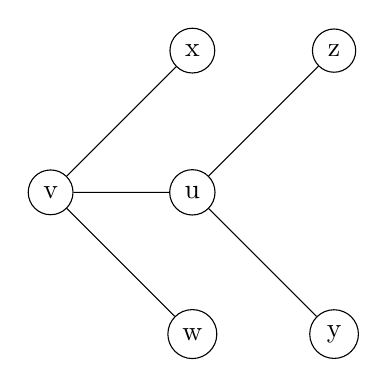
\begin{tikzpicture} 
	[main node/.style={circle, draw}, scale=1.8]
	\node[main node]  (v) at (0, 1) {v}; 
	\node[main node]  (w) at (1, 0) {w};
	\node[main node]  (u) at (1, 1) {u};
	\node[main node]  (x) at (1, 2) {x};
	\node[main node]  (y) at (2, 0) {y};
	\node[main node]  (z) at (2, 2) {z};
	\path (v) edge node {} (w);
	\path (v) edge node {} (u);
	\path (v) edge node {} (x);
	\path (u) edge node {} (y);
	\path (u) edge node {} (z);
	\end{tikzpicture}
	\label{fig:example_coverage}
	\caption{Coverage}
\end{figure}
\newline\underline{Stap \ref{itm:sort}}: Het eigenlijke sorteren van de SortedNodeArray gebeurt tijdens deze stap. De toppen worden gesorteerd in stijgende graad. Dit is een optimalisatie op het eigenlijke algoritme zodat het algoritme beter en sneller presteert. Deze SortedNodeArray heeft 3 methodes: toppen toevoegen, sorteren en de gesorteerde toppen opvragen. Dit zijn de enige vereisten. Het toevoegen van de toppen gebeurt tijdens het inlezen van de data en het sorteren van de toppen gebeurt \'{e}\'{e}nmalig bij het begin van het algoritme. Vervolgens kunnen de gesorteerde toppen altijd opgevraagd waarden verder in het algoritme, deze array verandert niet tijdens het algoritme. Enkel de coverage van de elementen is variabel. Als laatste wil ik de nadruk leggen op het feit dat deze stap een optimalisatie is. Het algoritme zou perfect werken, maar met iets slechtere prestaties zonder deze stap.
\newline\underline{Stap \ref{itm:degree1}}: Dit is ook een optimalisatie op het eigenlijke algoritme. Indien een top graad 1 heeft, weten we zeker dat de buur van deze top moet toegevoegd worden aan de dominante lijst aangezien de top enkel op deze manier bereikt kan worden. 
\newline\underline{Stap \ref{itm:actualalg}}: Deze stap voegt telkens toppen toe met een werkelijke bedekking groter dan een zeker getal. Dit getal start met 6 en decrementeert na elke iteratie van deze stap. Het algoritme zou ook werken indien er \'{e}\'{e}n iteratie is met minimum bedekking 1. Echter, het algoritme levert betere prestaties door eerst alle toppen toe te voegen die een hogere bedekking hebben, en vervolgens toppen met een kleinere bedekking.  Voor de duidelijkheid wordt het minimale algoritme, m.a.w. het algoritme die een dominante lijst produceert zonder de voorgaande optimalisaties, beschreven in algoritme \ref{alg:minimaldominantie}. Enkele belangrijke optimalisaties in het algoritme: 
\begin{itemize}
	\item Lijn \ref{step:opt1}: Als de coverage van de top gelijk is aan 0. Is het beter om bij een andere top lokaal te zoeken. 
	\item Lijn \ref{step:opt2}: Als de bedekking (bovengrens van de werkelijke bedekking) van een top 0 is, heeft het geen zin om deze top verder te bekijken. 
	\item Lijn \ref{step:opt3}: Als de werkelijke bedekking van een top gelijk is aan 0, heeft het ook geen zin om deze toe te voegen. 
\end{itemize}
Al deze optimalisaties verhinderen dat slechte toppen zouden toegevoegd worden. In het eigenlijke algoritme, wordt vergeleken in deze stappen met een minimum. Dit is echter niet nodig, maar zorgt wel voor betere prestaties. De enige vereiste van het algoritme is, dat de stap die beschreven wordt door algoritme \ref{alg:minimaldominantie} uitgevoerd wordt. In de implementatie wordt bij het bekijken van de nabuurschap van een top over de bogen ge\"{i}tereerd van de top. De top zelf bevat namelijk een List datastructuur die alle adjecente bogen bevat van de top. Ook wordt een variabele bijgehouden die het bereik van de dominante lijst bijhoudt. Zodra dit gelijk is aan $|V(G)|$ kan het algoritme eindigen. Als laatste wordt ook een boolean visited bijgehouden bij elke top. Een top wordt bezocht zodra hij of een buur wordt toegevoegd aan de dominante lijst. Eens een buur bezocht is, kan hij geen verdere bijdrage leveren tot het vergroten van het bereik van de dominante lijst. De implementatie van het bezoeken van een top verzekerd dat, indien een top nog niet bezocht werd, zijn coverage decrementeerd. 
\begin{tcolorbox}[blanker,float=btp, grow to left by=2cm,grow to right by=2cm]
	\begin{algoritme}
		\caption{Dominante verzameling van vlakke grafen}
		\begin{algorithmic}
			\Require Een planaire graaf G(V(G),E(G))
			\Ensure Een dominante verzameling D
			\State $totalCoverage \gets 0$
			\State $ i \gets 0$
			\While{$totalCoverage < |V(G)|$}
			\State $v \gets v_i \in V(G)$
			\If{$coverage(v) > 0$}\label{step:opt1}
			\State Neem $max\ |\ (\forall u \in \{v\} \cup N_G(v)) \land (max \ne u) \Rightarrow coverage(max)>coverage(u))$
			\If{$coverage(max) > 0$}\label{step:opt2}
			\State actualCoverage $\gets \{w\ |\ w  \in \{max\} \cup N_G(max) \land w\ niet \  bezocht\}$
			\If{$actualCoverage > 0$}\label{step:opt3}
			\State $totalCoverage \gets totalCoverage + actualCoverage$
			\State $coverage(max)  \gets 0$
			\State $ D \cup \{max\}$
			\State Bezoek max en zijn buren
			\EndIf 
			\EndIf
			\EndIf
			\State $i \gets i+1$
			\EndWhile		
		\end{algorithmic}
		\label{alg:minimaldominantie}
	\end{algoritme}
\end{tcolorbox}
\FloatBarrier
\subsubsection{Experimenten}
\paragraph{Optimalisaties}
Bij de experimenten omtrent optimalisaties gebruik ik steeds de gegeven testsets om het nut van een optimalisatie te testen. Er wordt (onder andere) vergeleken tussen een uitvoering zonder de optimalisatie en met de optimalisatie. De tabellen zijn telkens als volgt geformatteerd:
Bij de uitvoering van het algoritme onder de toestand beschreven in de bovenste kolommen heeft de graaf, gelezen uit graaf.sec, $x/y$\% toppen met x = $|D|$ (D = dominante lijst) en y = $|V(G)|$ Een cel is groen indien onder de huidige optie het algoritme de beste opties geeft voor graaf.sec. De exacte implementaties gebruik per algoritme kunnen gevonden worden in de Java-code.

\subparagraph{Sorteren} De variabele is hier de ordening van de toppen V(G) gebaseerd op hun graad. Er zijn 3 mogelijkheden: stijgende volgorde, dalende volgorde of willekeurige volgorde.  In tabel \ref{tabel:ordening} kan je zien dat bij elke graaf een dalende volgorde de beste resultaten teruggeeft. Een dalende volgorde betekent: indien we de toppen overloppen van index 0, worden de graad van elke top telkens kleiner. Aangezien deze optie de beste resultaten teruggeeft, wordt dit ook gebruikt. 



\subparagraph{Toppen met hoge minimumbedekking eerst}
Indien telkens opnieuw het algoritme uitgevoerd wordt, geeft dit betere resultaten als toppen met hogere minimum werkelijke bedekking eerst worden toegevoegd. Bij het eerste experimenten testen we wanneer het algoritme het beste presteert als telkens eerst toppen met een zekere werkelijke bedekking worden toegevoegd, en dit iteratief gebeurt met decrementerende minimale werkelijke bedekking. Graaf5.sec tot graaf8.sec laten we hier buiten beschouwing aangezien deze telkens even goed presteren. In tabel \ref{tabel:bedekking1} en \ref{tabel:bedekking2} zie je de resultaten van het uitvoeren van het algoritme vanaf een zekere werkelijke bedekking. De prestatie van een zekere minimale bedekking is zeer variabel van graaf tot graaf, het gemiddelde balanceert rond beginnen met een minimale bedekking van 7. Uit tabel \ref{tabel:bedekking3} kan geconcludeerd worden dat minimale bedekking 6 in het geheel de beste minimale dominante verzamelingen levert. Dit optimalisatieniveau wordt ook gebruikt in het algoritme.

\subparagraph{Toppen met graad 1}
In dit experiment wordt getest wat het effect is van het vooraf toevoegen van buren met toppen van graad 1. Hierbij worden de optimale instellingen verkregen uit vorige experimenten gebruikt. In tabel \ref{table:oneneighbour} kunnen de resultaten bekeken worden van het experiment. De optimalisatie zorgt telkens voor betere resultaten. Vooral bij graaf5.sec tot en met graaf8.sec is er een merkwaardig verschil. De grafen kunnen hier namelijk volledig opgebouwd worden door het toevoegen van de buren van toppen met graad 1. Deze optimalisatie is dus zeker helpvol en kan veel onnodig rekenwerk besparen.

\subparagraph{Niet-lineair gretig algoritme}
Als laatste bekijk ik het effect van het gebruik van een bovengrens (benadering) van de werkelijke coverage. Hiervoor heb ik het algoritme ge\"{i}mplementeerd, maar in de plaats van getCoverage() wordt nu getActualCoverage() gebruikt. Dit is de som van het aantal onbezochte buren en zichzelf indien de top nog niet bezocht werd. Op figuur \ref{tabel:nonlinear} kan je zien dat het algoritme weliswaar altijd minstens even goed presteert. Het verschil is echter merkwaardig klein. Het niet-lineaire algoritme presteert hoogstens 0.5\% beter. 

\begin{table}
	\centering
	\begin{tabular}{|l|c|c|c|}
		\hline
		& \multicolumn{3}{c|}{Ordening}		\\ \hline
		Graaf & Geen ordening  & Stijgende volgorde  & Dalende volgorde 		\\ \hline
		graaf1.sec & 20,44\% & 20,55\% &  \cellcolor{LimeGreen}19,98\%		\\ \hline
		graaf2.sec & 19,04\% & 19,02\% &  \cellcolor{LimeGreen}18,64\%		\\ \hline
		graaf3.sec & 21,10\% & 20,98\% &  \cellcolor{LimeGreen}20,87\%		\\ \hline
		graaf4.sec & 19,80\% & 19,76\% &  \cellcolor{LimeGreen}19,48\%		\\ \hline
		graaf5.sec &  \cellcolor{LimeGreen}33,33\% & 33,33\% & 33,33\%		\\ \hline
		graaf6.sec &  \cellcolor{LimeGreen}33,33\% & 33,33\% & 33,33\%		\\ \hline
		graaf7.sec &  \cellcolor{LimeGreen}33,33\% & 33,33\% & 33,33\%		\\ \hline
		graaf8.sec &  \cellcolor{LimeGreen}33,33\% & 33,33\% & 33,33\%		\\ \hline
		triang1.sec & 17,16\% & 17,09\% &  \cellcolor{LimeGreen}16,72\%		\\ \hline
		triang2.sec & 16,90\% & 16,77\% &  \cellcolor{LimeGreen}16,58\%		\\ \hline
	\end{tabular}
	\caption{Ordening van de toppen}
	\label{table:ordening}
\end{table}

\begin{table}
	\centering
	\begin{tabular}{|l|c|c|c|c|c|c|c|c|}
		\hline
		& \multicolumn{8}{c|}{Minimum Bedekking}		\\ \hline
		Graaf & 0  & 1  & 2  & 3  & 4  & 5  & 6  & 7 		\\ \hline
		graaf1.sec & 22,39\% & 20,98\% & 20,38\% & 20,06\% & 20,05\% &  \cellcolor{LimeGreen}19,98\% & 19,98\% & 20,00\%		\\ \hline
		graaf2.sec & 21,10\% & 19,82\% & 19,24\% & 18,92\% & 18,70\% & 18,66\% &  \cellcolor{LimeGreen}18,64\% & 18,66\%		\\ \hline
		graaf3.sec & 23,27\% & 21,81\% & 21,22\% & 20,99\% & 20,92\% & 20,89\% & 20,87\% &  \cellcolor{LimeGreen}20,84\%		\\ \hline
		graaf4.sec & 21,81\% & 20,61\% & 20,01\% & 19,70\% & 19,54\% & 19,49\% &  \cellcolor{LimeGreen}19,48\% & 19,50\%		\\ \hline
		graaf5.sec &  \cellcolor{LimeGreen}33,33\% & 33,33\% & 33,33\% & 33,33\% & 33,33\% & 33,33\% & 33,33\% & 33,33\%		\\ \hline
		graaf6.sec &  \cellcolor{LimeGreen}33,33\% & 33,33\% & 33,33\% & 33,33\% & 33,33\% & 33,33\% & 33,33\% & 33,33\%		\\ \hline
		graaf7.se c &  \cellcolor{LimeGreen}33,33\% & 33,33\% & 33,33\% & 33,33\% & 33,33\% & 33,33\% & 33,33\% & 33,33\%		\\ \hline
		graaf8.sec &  \cellcolor{LimeGreen}33,33\% & 33,33\% & 33,33\% & 33,33\% & 33,33\% & 33,33\% & 33,33\% & 33,33\%		\\ \hline
		triang1.sec & 19,03\% & 17,82\% & 17,25\% & 17,06\% & 16,86\% & 16,75\% & 16,72\% &  \cellcolor{LimeGreen}16,69\%		\\ \hline
		triang2.sec & 18,81\% & 17,67\% & 17,15\% & 16,85\% & 16,71\% & 16,61\% & 16,58\% &  \cellcolor{LimeGreen}16,57\%		\\ \hline
	\end{tabular}
	\caption{Minimale bedekking van de toppen.}
	\label{tabel:bedekking1}
\end{table}

\begin{table}[tbp]
	\centering
	\begin{tabular}{|l|c|c|c|c|c|c|c|c|}
		\hline
		& \multicolumn{8}{c|}{Minimum Bedekking}		\\ \hline
		Graaf & 8  & 9  & 10  & 11  & 12  & 13  & 14  & 15 		\\ \hline
		graaf1.sec &  \cellcolor{LimeGreen}20,13\% & 20,18\% & 20,22\% & 20,24\% & 20,22\% & 20,19\% & 20,19\% & 20,19\%		\\ \hline
		graaf2.sec & 18,70\% &  \cellcolor{LimeGreen}18,69\% & 18,70\% & 18,71\% & 18,71\% & 18,70\% & 18,69\% & 18,70\%		\\ \hline
		graaf3.sec &  \cellcolor{LimeGreen}20,78\% & 20,80\% & 20,82\% & 20,82\% & 20,81\% & 20,78\% & 20,78\% & 20,78\%		\\ \hline
		graaf4.sec & 19,51\% & 19,50\% &  \cellcolor{LimeGreen}19,49\% & 19,51\% & 19,51\% & 19,50\% & 19,49\% & 19,50\%		\\ \hline
		graaf5.sec &  \cellcolor{LimeGreen}33,33\% & 33,33\% & 33,33\% & 33,33\% & 33,33\% & 33,33\% & 33,33\% & 33,33\%		\\ \hline
		graaf6.sec &  \cellcolor{LimeGreen}33,33\% & 33,33\% & 33,33\% & 33,33\% & 33,33\% & 33,33\% & 33,33\% & 33,33\%		\\ \hline
		graaf7.sec &  \cellcolor{LimeGreen}33,33\% & 33,33\% & 33,33\% & 33,33\% & 33,33\% & 33,33\% & 33,33\% & 33,33\%		\\ \hline
		graaf8.sec &  \cellcolor{LimeGreen}33,33\% & 33,33\% & 33,33\% & 33,33\% & 33,33\% & 33,33\% & 33,33\% & 33,33\%		\\ \hline
		triang1.sec &  \cellcolor{LimeGreen}16,73\% & 16,76\% & 16,77\% & 16,76\% & 16,75\% & 16,74\% & 16,75\% & 16,76\%		\\ \hline
		triang2.sec & 16,57\% & 16,56\% & 16,56\% & 16,55\% & 16,54\% & 16,52\% & 16,53\% &  \cellcolor{LimeGreen}16,52\%		\\ \hline
	\end{tabular}
	\caption{Minimale bedekking van de toppen.}
	\label{tabel:bedekking2}
\end{table}

\begin{table}
	\centering
	\begin{tabular}{|c|c|}
		\hline
		Minimum bedekking & $|D|\ /\ |V(G)|$		\\ \hline
		0 & 25,0729\% \\ \hline
		1 & 24,2659\% \\ \hline
		2 & 23,8922\% \\ \hline
		3 & 23,6965\% \\ \hline
		4 & 23,5913\% \\ \hline
		5 & 23,5475\% \\ \hline
		6 &\cellcolor{LimeGreen} 23,5370\% \\ \hline
		7 & 23,5413\% \\ \hline
		8 & 23,5541\% \\ \hline
		9 & 23,5519\% \\ \hline
	\end{tabular}
	\caption{Aantal toppen in alle dominante verzamelingen t.o.v. aantal toppen in alle grafen.}
	\label{tabel:bedekking3}
\end{table}

\begin{table}
	\centering
	\begin{tabular}{|l|c|c|}
		\hline
		& \multicolumn{2}{c|}{Toppen van graad 1}		\\ \hline
		Graaf & Zonder optimalisatie  & Met optimalisatie 		\\ \hline
		graaf1.sec & 20,03\% &  \cellcolor{LimeGreen}19,98\%		\\ \hline
		graaf2.sec & 18,66\% &  \cellcolor{LimeGreen}18,64\%		\\ \hline
		graaf3.sec & 21,01\% &  \cellcolor{LimeGreen}20,87\%		\\ \hline
		graaf4.sec & 19,60\% &  \cellcolor{LimeGreen}19,48\%		\\ \hline
		graaf5.sec & 38,72\% &  \cellcolor{LimeGreen}33,33\%		\\ \hline
		graaf6.sec & 38,65\% &  \cellcolor{LimeGreen}33,33\%		\\ \hline
		graaf7.sec & 38,67\% &  \cellcolor{LimeGreen}33,33\%		\\ \hline
		graaf8.sec & 38,60\% &  \cellcolor{LimeGreen}33,33\%		\\ \hline
		triang1.sec &  \cellcolor{LimeGreen}16,72\% & 16,72\%		\\ \hline
		triang2.sec &  \cellcolor{LimeGreen}16,58\% & 16,58\%		\\ \hline
	\end{tabular}
	\caption{Experiment met betrekking tot het al dan niet toevoegen van buren van toppen met graad 1.}
	\label{table:oneneighbour}
\end{table}

\begin{table}
	\centering
	\begin{tabular}{|l|c|c|}
		\hline
		& \multicolumn{2}{c|}{Vergelijking lineair - niet lineair gretig algoritme}		\\ \hline
		Graaf & Niet-lineair  & Lineair 		\\ \hline
		graaf1.sec &  \cellcolor{LimeGreen}19,57\% & 19,98\%		\\ \hline
		graaf2.sec &  \cellcolor{LimeGreen}18,16\% & 18,64\%		\\ \hline
		graaf3.sec &  \cellcolor{LimeGreen}20,50\% & 20,87\%		\\ \hline
		graaf4.sec &  \cellcolor{LimeGreen}19,05\% & 19,48\%		\\ \hline
		graaf5.sec &  \cellcolor{LimeGreen}33,33\% & 33,33\%		\\ \hline
		graaf6.sec &  \cellcolor{LimeGreen}33,33\% & 33,33\%		\\ \hline
		graaf7.sec &  \cellcolor{LimeGreen}33,33\% & 33,33\%		\\ \hline
		graaf8.sec &  \cellcolor{LimeGreen}33,33\% & 33,33\%		\\ \hline
		triang1.sec &  \cellcolor{LimeGreen}16,47\% & 16,72\%		\\ \hline
		triang2.sec &  \cellcolor{LimeGreen}16,17\% & 16,58\%		\\ \hline
	\end{tabular}
	\caption{Vergelijking implementaties}
	\label{tabel:nonlinear}
\end{table}

\paragraph{Verschillende grafen}
In dit onderdeel ga ik in op enkele voorbeeldgrafen en bespreek ik hoe het algoritme presteert bij de gegeven grafen. 

De worst case graaf voor dominante verzamelingen is een \underline{cyclische graaf}, zodat elke top juist 2 bogen heeft en de graaf juist 1 cykel bevat. 
Elke top heeft dus graad 2. Een minimale dominante verzameling bevat dan 1/3 van de toppen van de graaf. Bij het uitvoeren van mijn algoritme op dergelijke graaf, geeft het altijd de optimale dominante verzameling terug met grootte 1/3, hier werkt het algoritme dus perfect. 
Als volgt kijken we naar grafen waarvan de buren op afstand 2 van een ideale top een groot aantal toppen heeft. Aangezien de bedekking van deze toppen niet aangepast worden door het toevoegen van een top op afstand 2, zou dit een slechtere benadering moeten geven. Een goed voorbeeld hiervan is een \underline{Petersen-graaf}. Dit is een graaf met 10 toppen en 15 bogen en wordt vaak gebruikt als tegenvoorbeeld voor vele optimistische problemen. Bij het uitvoeren van het algoritme op deze graaf, bekom ik een dominante verzameling met 3 toppen, opnieuw presteert het ideaal. 
Als laatste ik de graaf die je kan zien op figuur \ref{fig:schaakmat}
, ik benoem de graaf als de \underline{schaakmat graaf}. Het is een graaf met 8x8 toppen zodat elke top een vak uit het speelveld van een schaakmat voorstelt, en de toppen van 2 naburige vakjes verbonden zijn door een boog. Het is goed mogelijk dat mijn algoritme voor deze graaf slecht presteert, aangezien alle toppen zeer verbonden zijn, zodat de coverage een slechte benadering zal geven. De coverage van de buren op afstand 2 van een top zullen immers niet aangeraakt worden. Dit zorgt ervoor dat de dominante lijst slechtere resultaten zal bekomen. Het resultaat van mijn algoritme op de gegeven graaf kan je ook zien op figuur \ref{fig:schaakmat}. De toppen uit de dominante lijst werden in het groen gekleurd. De dominante lijst bevat $22/64$ (34\%) van de toppen. Het is moeilijk om voor een graaf van deze omvang te weten of de oplossing een goede benadering heeft. Het is makkelijker om de graaf op te delen in 4x4 vlakken. Beschouw figuur \ref{fig:schaakmat2}, een minimale dominante verzaleming wordt verkregen door de groene toppen. Dit zijn er precies 6. 
Een dominante verzameling voor een schaakmatgraaf, zou dan kunnen verkregen worden door in elke vlak juist die 4 toppen te kiezen. Dan is er een dominante verzameling van 24 toppen. Dit is een slechtere benadering dan dan de benadering van het algoritme. Een echte optimale verzameling zoeken van een graaf van dergelijke omvang is moeilijk, daarom implementeerde ik een variatie op mijn algoritme, die niet lineair werkt, maar betere benaderingen moet geven. De wijziging op het algoritme is als volgt: in de plaats van een bovengrens van de werkelijke coverage te gebruiken, wordt nu de echte coverage gebruikt zodat we in elke stap verzekeren dat de beste lokale top toegevoegd wordt. Bij het uitvoeren van het algoritme op de schaakmat graaf krijg ik een verzameling van 21 toppen. Dit is slechts 1 top minder dan het lineaire algoritme. We kunnen dus stellen dat het algoritme goede benaderingen geeft. 

\begin{figure}[tbp]
	\centering
	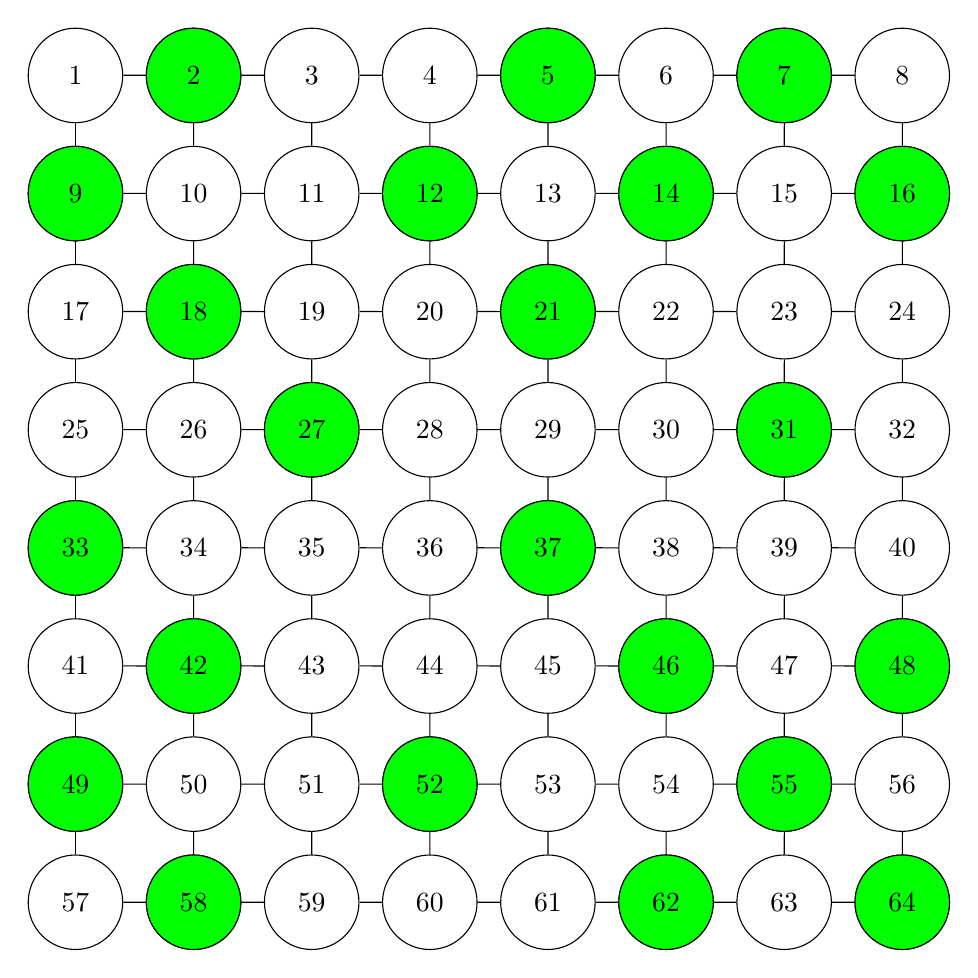
\begin{tikzpicture} 
	[main node/.style={circle, draw}, minimum width=1.2cm, minimum height=1.2cm, scale=1.5]
	\newcounter{x}
	\foreach \i in {0,1,...,7}{
		\foreach \j in {0,1,...,7}{
			\stepcounter{x};
			\node[main node]  (\arabic{x}) at (\j, 8-\i) {\arabic{x}};
		}
	}

	\setcounter{x}{8}
	\newcounter{y}
	\newcounter{z}
	\stepcounter{z}
	\foreach \i in {1,2,...,7}{
		\foreach \j in {1,2,...,7}{
			\stepcounter{y};
			\stepcounter{z};
			\stepcounter{x};
			\path (\arabic{y}) edge node {} (\arabic{z}); %right
			\path (\arabic{y}) edge node {} (\arabic{x}); %down
		}
		\stepcounter{y};
		\stepcounter{z};
		\stepcounter{x};
	}

	\setcounter{x}{57}
	\setcounter{y}{58}
	\newcounter{a}
	\newcounter{b}
	\setcounter{a}{8}
	\setcounter{b}{16}
	\foreach \i in {1,2,...,7}{
		\path (\arabic{x}) edge node {} (\arabic{y}); %right
		\path (\arabic{a}) edge node {} (\arabic{b}); %down
		\stepcounter{y};
		\stepcounter{x};
		\addtocounter{a}{8};
		\addtocounter{b}{8};
	}	
	
	%color dominant list nodes.
	\node[main node, fill=green] (55) at (6,2) {55};
	\node[main node, fill=green] (52) at (3,2) {52};
	\node[main node, fill=green] (42) at (1,3) {42};
	\node[main node, fill=green] (31) at (6,5) {31};
	\node[main node, fill=green] (18) at (1,6) {18};
	\node[main node, fill=green] (14) at (5,7) {14};
	\node[main node, fill=green] (37) at (4,4) {37};
	\node[main node, fill=green] (12) at (3,7) {12};
	\node[main node, fill=green] (58) at (1,1) {58};
	\node[main node, fill=green] (2) at (1,8) {2};
	\node[main node, fill=green] (16) at (7,7) {16};
	\node[main node, fill=green] (27) at (2,5) {27};
	\node[main node, fill=green] (62) at (5,1) {62};
	\node[main node, fill=green] (48) at (7,3) {48};
	\node[main node, fill=green] (33) at (0,4) {33};
	\node[main node, fill=green] (64) at (7,1) {64};
	\node[main node, fill=green] (49) at (0,2) {49};
	\node[main node, fill=green] (7) at (6,8) {7};
	\node[main node, fill=green] (9) at (0,7) {9};
	\node[main node, fill=green] (5) at (4,8) {5};
	\node[main node, fill=green] (46) at (5,3) {46};
	\node[main node, fill=green] (21) at (4,6) {21};
	\end{tikzpicture}
	\caption{Een schaakmatgraaf}
	\label{fig:schaakmat}
\end{figure}

\begin{figure}[tbp]
	\centering
	\begin{tikzpicture} 
	[main node/.style={circle, draw}, minimum width=1.2cm, minimum height=1.2cm, scale=1.5]
	\setcounter{x}{0}
	\foreach \i in {0,1,...,3}{
		\foreach \j in {0,1,...,3}{
			\stepcounter{x};
			\node[main node]  (\arabic{x}) at (\j, 4-\i) {\arabic{x}};
		}
	}
	
	\setcounter{x}{4}
	\setcounter{y}{0}
	\setcounter{z}{1}
	\foreach \i in {1,2,3}{
		\foreach \j in {1,2,3}{
			\stepcounter{y};
			\stepcounter{z};
			\stepcounter{x};
			\path (\arabic{y}) edge node {} (\arabic{z}); %right
			\path (\arabic{y}) edge node {} (\arabic{x}); %down
		}
		\stepcounter{y};
		\stepcounter{z};
		\stepcounter{x};
	}
	
	\setcounter{x}{13}
	\setcounter{y}{14}
	\setcounter{a}{4}
	\setcounter{b}{8}
	\foreach \i in {1,2,3}{
		\path (\arabic{x}) edge node {} (\arabic{y}); %right
		\path (\arabic{a}) edge node {} (\arabic{b}); %down
		\stepcounter{y};
		\stepcounter{x};
		\addtocounter{a}{4};
		\addtocounter{b}{4};
	}	
	\node[main node, fill=green] (1) at (0,4) {1};
	\node[main node, fill=green] (6) at (1,3) {6};
	\node[main node, fill=green] (11) at (2,2) {11};
	\node[main node, fill=green] (16) at (3,1) {16};
	\node[main node, fill=green] (4) at (3,4) {4};
	\node[main node, fill=green] (13) at (0,1) {13};
	
	\end{tikzpicture}
	\caption{Een 4x4 schaakmatgraaf}
	\label{fig:schaakmat2}
\end{figure}

\paragraph{Conlusie}
Desondanks het feit dat dit algoritme werkt met benaderingen voor de werkelijke bedekking, presteert het bijna even goed als een algoritme waarbij gewerkt wordt met werkelijke bedekkingen. Ook is het zeer moeilijk om een graaf te vinden waarbij het algoritme faalt. Ik denk dus dat het moeilijk is om een gretig lineair algoritme te vinden die veel beter presteert dan het huidige algoritme. 


\end{document}
